\chapter{Simulation of hard-sphere fluids}
Several methods exist for simulating fluids 
consisting of rigid spheres. They can be 
divided into two categories, namely Monte 
Carlo (MC) models, and molecular dynamics 
(MD) models. MC methods sample statistical 
ensembles using random walk,  % TODO: Find a better term than random walk.
while MD methods use Newton's equations of 
motion to compute the deterministic path 
of a large collection of particles.

Monte Carlo methods are typically easier to 
use with hard-sphere potentials, but can not 
be used to compute transport coefficients. 
% Can't, or can with difficulty? 
% That's an important distinction.
Molecular dynamics methods on the other 
hand, allow calculating dynamical and 
out-of-equilibrium properties of a system. 
To compute the viscosity of a system, 
MD methods should therefore be used. 

This section therefore gives an introduction 
to molecular dynamics, focusing especially on 
molecular dynamics for hard and pseudo-hard 
spheres \cite{ref:allen:MD_sim}.

% Mer generelt om MD (inkl hendelsesdrevent)
\section{Event-driven molecular dynamics simulation}
A simple method for performing molecular 
dynamics simulations with hard sphere in 
is an \emph{event-driven simulation}. 
Key elements of this simulation method 
is outlined below.

Compute the time until a collision occurs, for all particles in the system.
All collisions are stored in a list containing at least information about
the time of the collision, and the identity of the two involved particles.
Then, the time until the earliest collision is identified by searching through the list.
Using Newton's equations of motion, all atoms are propagated freely until
the collision happens.
Through conservation laws, the colliding particles' velocities are then updated.
Their next collisions are then added to the list of upcoming collisions.
This process is repeated, and all atom positions are updated with the time 
until the next collision in the list.

It should be noted that after a collision happens, other collisions involving
either of the two particles will be invalid.
These should be discarded from the list.

\section{Continuous potential MD simulation methods}
Several powerful and efficient molecular dynamics 
programmes are easily available, including LAMMPS, 
GROMACS, DL\_POLY and NAND. % TODO add references.  
These do, however, not handle discontinuous potentials.
Thus, the event-driven method is not supported by 
any of these programmes \cite{ref:allen:MD_sim}. In 
order to utilize the efficiency of the available MD 
software, it is more convenient to use a different 
method. The hard sphere potential can be approximated 
with a steep but continuous interaction potential 
instead. Then, the particle positions are updated 
using numerical integration methods with short, 
finite time steps.

Additionally, once there are long-range 
interaction forces between particles, then 
interactions occur at all times. In this 
case, the event driven simulation does not 
work, and integration methods are required. 
Therefore, continuous potential modelling 
is much more useful for realistic fluid models.

Several potentials are possible to use as 
hard-sphere approximations. The Lennard-Jones 
potential 
\[
    \label{eq:lennard_jones_potential}
    u_{\text{LJ}}(r) = 
        4 \epsilon \left[
            \left(\frac{\sigma}{r}\right)^{12} -
            \left(\frac{\sigma}{r}\right)^{6}
        \right]
\]
is a well-known example of historical importance.
Here, $\epsilon$ is the well depth -- the minimal value of 
the potential. As in \eqref{eq:hard_sphere_potential}, 
$\sigma$ and $r$ are the diameter and relative distance of 
the interacting particles.

If the attractive part, 
$\left[- \left(\frac{\sigma}{r}\right)^{6}\right]$
in equation \eqref{eq:lennard_jones_potential} 
is removed from the potential, then $u_{\text{LJ}}(r)$ 
can represent purely repulsive interactions. This is done 
by shifting the potential upwards by its minimal value 
$\epsilon$ and cutting it off there. Thus, the potential 
is exactly zero once it has reached its minimum. The 
resulting potential
\[
    \label{eq:WCA_potential}
    u_{WCA}(r) = 
    \begin{cases}
        4 \epsilon \left[
            \left(\frac{\sigma}{r}\right)^{12} -
            \left(\frac{\sigma}{r}\right)^{6}
        \right]
        + \epsilon,
            & r < 2^\frac{1}{6} \sigma\\
        0,  & r > 2^\frac{1}{6}\sigma.
    \end{cases}
\]
is known as a WCA-potential.
This serves as an approximation to a hard sphere potential.
% This is explained below. 
% TODO: Move the explanation here, so that everything is chronological.

Increased computer efficiency makes it more appropriate 
to use steeper potentials than the WCA-potential.
In particular, Jover et al. \cite{ref:jover:pseudo_hard} 
has proposed the Mie (or generalized Lennard-Jones) potential
\[
    u_{\text{Mie}}(r) = 
        \frac{\lambda_r}{\lambda_r - \lambda_a}
        \left(\frac{\lambda_r}{\lambda_a}\right)
        ^{\frac{\lambda_a}{\lambda_r - \lambda_a}}
        \epsilon \left[
            \left(\frac{\sigma}{r}\right)^{\lambda_r} -
            \left(\frac{\sigma}{r}\right)^{\lambda_a}
        \right],
\]
as an approximation to the hard-sphere interaction potential.
% What's a better word than "strength"??
The exponents $\lambda_r$ and $\lambda_a$ define the strength 
of the repulsive and attractive parts of the potential.

Cutting and shifting the $u_{\text{Mie}}$ 
potential as done in equations
\eqref{eq:lennard_jones_potential} 
and \eqref{eq:WCA_potential}, gives 
the steep non-negative WCA potential 
\[
    u_{(\lambda_a, \lambda_b)}(r) = 
    \begin{cases}
        \frac{\lambda_r}{\lambda_r - \lambda_a}
        \left(\frac{\lambda_r}{\lambda_a}\right)
        ^{\frac{\lambda_a}{\lambda_r - \lambda_a}}
        \epsilon \left[
            \left(\frac{\sigma}{r}\right)^{\lambda_r} -
            \left(\frac{\sigma}{r}\right)^{\lambda_a}
        \right]
        + \epsilon,
            & r < \sigma \left(
                \frac{\lambda_r}{\lambda_a}
            \right)^\frac{1}{\lambda_r - \lambda_a} \\
        0,  & r > \sigma \left(
                \frac{\lambda_r}{\lambda_a}
            \right)^\frac{1}{\lambda_r - \lambda_a},
    \end{cases}
\]
closely resembling that of an infinitely steep hard 
wall potential (equation \eqref{eq:hard_sphere_potential}).
This potential is referred to as a pseudo hard-sphere 
(PHS) potential.

Jover et al. chose the exponents \((\lambda_r, \lambda_a) = (50, 49)\), 
as a compromise between faithfulness of the pseudo 
hard representation towards the perfectly hard 
wall, and computational speed. Higher exponents 
will produce a steeper repulsion. This however, 
comes at a cost.  The steeper the potential, the 
shorter time steps are needed to ensure that the 
computations are precise. % TODO: Definer hva presist betyr.
Therefore, steeper repulsions are computationally 
more expensive to simulate.

Writing it out for clarity, the WCA 
(50, 49)-potential has the form
\[
    u_{(50, 49)}(r) = 
    \begin{cases}
        50
        \left(\frac{50}{49}\right)^{49}
        \epsilon \left[
            \left(\frac{\sigma}{r}\right)^{50} -
            \left(\frac{\sigma}{r}\right)^{49}
        \right]
        + \epsilon,
            & r < \frac{50}{49} \sigma\\
        0,  & r > \frac{50}{49} \sigma.
    \end{cases}
\]

\begin{figure}[htbp]
    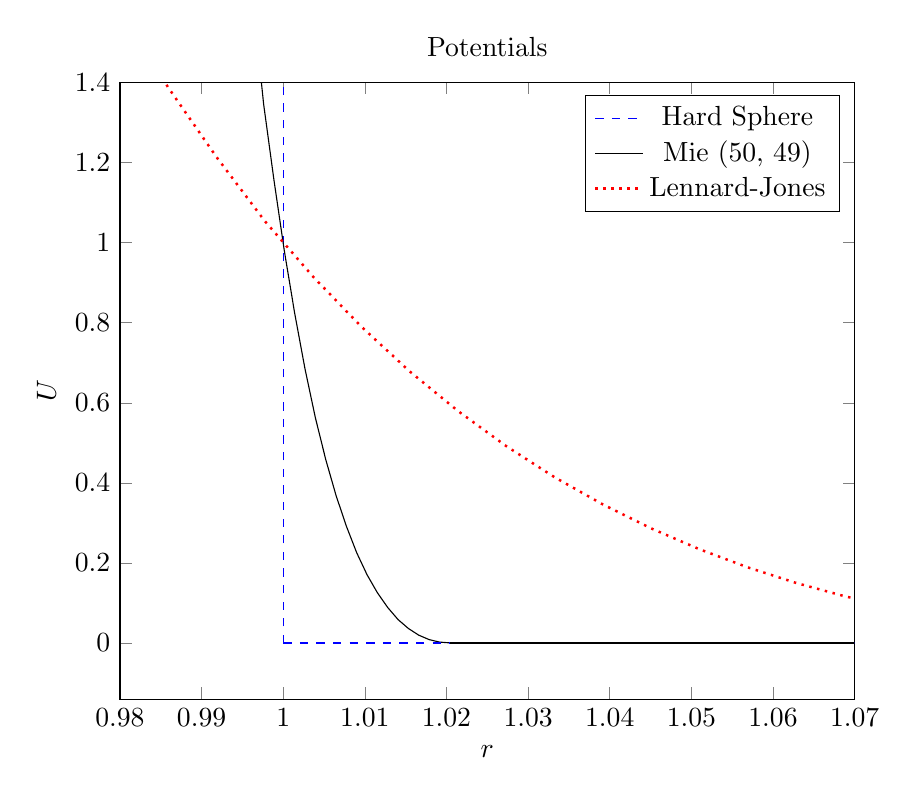
\begin{tikzpicture}
    \begin{axis}[
        title=Potentials,
        xlabel=$r$,
        ylabel=$U$,
        width=0.9\textwidth,
        ymax=1.4,
        xmin=0.98,
        xmax=1.07,
        cycle list = {
            color=blue,     style=dashed,   \\%
            color=black,    style=solid,    \\%
            color=red,      style=dotted,   line width=0.9pt,\\%
}
    ]
        % HARD SPHERE:
        \addplot+ [
            domain=0:1.1,
            mark=none,
            ] coordinates {(1,0) (1,2)};
            \addlegendentry{Hard Sphere}
        % MIE:
        \addplot+ [
            domain=0.99:1.0204,
            ]{50*(50/49)^49 * ((1/x)^50 - (1/x)^49) + 1.0};
            \addlegendentry{Mie (50, 49)}
        % LENNARD-JONES
        \addplot+ [
            domain=0.98:1.122,
        ]{4*((1/x)^12 - (1/x)^6) + 1};
        \addlegendentry{Lennard-Jones}
        % HARD SPHERE:
        \addplot+ [
            domain=1:1.1,
            mark=none,
        ] {0};
        % MIE:
        \addplot+ [
            color=black,
            domain=1.0204:1.1,
        ]{0};
        % LENNARD-JONES
        \addplot+ [
            domain=1.122:1.2,
        ]{0};
    \end{axis}
\end{tikzpicture}

    \caption{The cut-and-shifted WCA(50, 49)-potential 
            compared to the cut and shifted WCA(12, 6) 
            (Lennard-Jones) as well as the hard sphere 
            potential.
    }
\end{figure}

Pousaneh and de Wijn \cite{ref:pousaneh:shear_viscosity} 
have shown that such a pseudo-hard sphere potential 
can be used to model viscosity for a one-component hard-sphere fluid, 
and that the obtained viscosity is in agreement with Enskog theory.
% However, to the best of our knowledge, such a confirmation has not 
% been published for fluids of more than one component. 
% C: Dette er er ikke sjekket, men er jo delvis det du skal gjøre.


\section{Measuring the viscosity of a fluid in NEMD}
\label{sec:theory:muller_plathe}
Müller-Plathe \cite{ref:mullerplathe:reversing_the_perturbation} 
has proposed a method of computing the viscosity of a fluid in 
nonequilibrium molecular dynamics (NEMD) simulations.
% TODO: Describe method, including figures.

Consider a rectangular box with sides of length \((L_x, L_y, L_z)\) 
with periodic boundary conditions.
The box contains a hard sphere fluid at equilibrium.
We divide the system into two equal slabs, their border 
being parallel to the $xy$-plane at height \(z = L_z/2\).
Now, we can define three parallel planes, at 
\(z = \{0, L_z/2, L_z\}\), which are the edges of the two slabs.
At these edges, we will control the velocity of the particles, 
making sure that the particles flow in the directions
\[
    \label{eq:velocity_directions}
    \hat{u}_x(z) =
    \begin{cases}
        +\hat{x}, \,z = L_z,    \\
        -\hat{x}, \,z = L_z/2,  \\
        +\hat{x}, \,z = 0,    \\
    \end{cases}
\]
as shown in figure (??). %TODO: Figure.
Here, \(u_x(z)\) denotes the average velocity component 
in $x$-direction, of the particles at height $z$.
The hat ``\(\,\, \hat{ } \,\,\)'' denotes 
directional vectors of length unity.

The particle flows are adjusted through an unphysical process known as a 
\textbf{reverse perturbation}\cite{ref:mullerplathe:reversing_the_perturbation},
as follows:

Find the particle in the \(z = 0\) slab edge with the lowest 
(most negative) velocity component in the \(+x\)-direction.
Correspondingly, find the particle in the \(z = L/2\) border 
with the largest velocity component in the \(+x\)-direction.
Then, swap the momenta of these two particles.
Repeat the process for the top slab, swapping the smallest momentum 
in the \(z = L\) edge with the largest momentum in the \(z = L/2\) edge.
This process is then repeated periodically.
The repeated reverse perturbations cause a velocity profile in the fluid,
as shown in figure (??). % TODO: Figure.
At the edges of the slabs, the velocity directions 
is given by equation \eqref{eq:velocity_directions}.

The velocity profile will cause a momentum flux in $z$-direction,
\[
    \label{eq:momentum_flux}
    j_z = -\eta \frac{\partial u_x}{\partial z}.
\]
This flux is proportional to the viscosity of the fluid, and is measurable.
Thus, the viscosity can be calculated from velocity data generated in the 
MD simulation.

\begin{figure}
    \begin{center}
        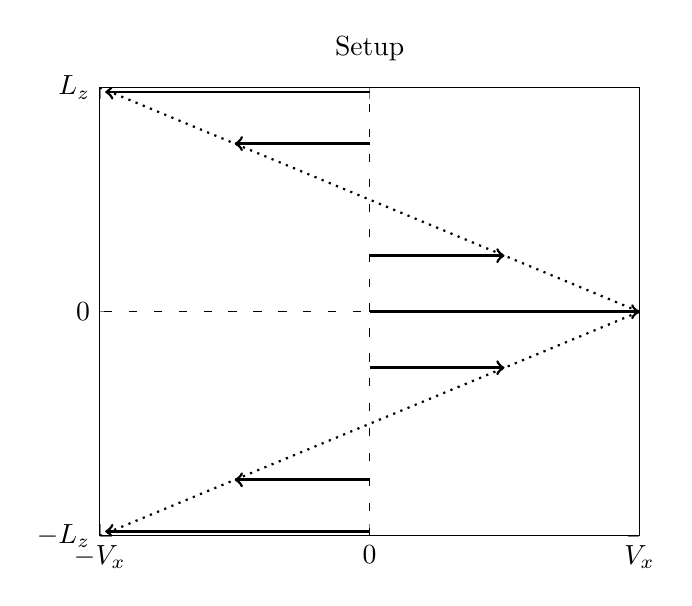
\begin{tikzpicture}
\def\V{1.0}
\def\Lz{1.0}
\begin{axis}[
    title=Setup,
    xmin=-\V,
    xmax=\V,
    ymin=-1.00*\Lz,
    ymax=1.00*\Lz,
    xtick={-\V,0,\V},
    ytick={-\Lz,0,\Lz},
    xticklabels={$-V_x$, $0$, $V_x$},
    yticklabels={$-L_z$, $0$, $L_z$},
]
    \addplot[ % Upper half velocity profile
        domain=-\V:\V,
        dotted,
        line width=0.8pt,
        ] {-\Lz/(2*\V)*x+\Lz/2};
    \addplot[ % Lower half velocity profile
        domain=-\V:\V,
        dotted,
        line width=0.8pt,
        ] {\Lz/(2*\V)*x-\Lz/2};
    \addplot[ % Middle plane of box
        domain=-2*\V:2*\V,
        loosely dashed,
        ] {0};
    \addplot[ % Middle plane of box
        loosely dashed,
        ] coordinates {(0,-2*\Lz) (0,2*\Lz)};
        \draw [-to, line width=1pt] (0, 0.25)   -- (0.5,    0.25);
        \draw [-to, line width=1pt] (0, -0.25)  -- (0.5,    -0.25);

        \draw [-to, line width=1pt] (0, 0.75)   -- (-0.5,   0.75);
        \draw [-to, line width=1pt] (0, -0.75)  -- (-0.5,   -0.75);

        \draw [-to, line width=1pt] (0, 0.98)      -- (-0.98,   0.98);
        \draw [-to, line width=1pt] (0, -0.98)     -- (-0.98,   -0.98);

        \draw [-to, line width=1pt] (0, 0)      -- (1.0,   0);
\end{axis}
\end{tikzpicture}

        \caption{The setup of the Müller-Plathe experiment.}
    \end{center}
\end{figure}

